\documentclass[
  bibliography=totoc,     % Literatur im Inhaltsverzeichnis
  captions=tableheading,  % Tabellenüberschriften
  titlepage=firstiscover, % Titelseite ist Deckblatt
  parskip=half,
]{scrartcl}

% Paket float verbessern
\usepackage{scrhack}

% Warnung, falls nochmal kompiliert werden muss
\usepackage[aux]{rerunfilecheck}

% unverzichtbare Mathe-Befehle
\usepackage{amsmath}
% viele Mathe-Symbole
\usepackage{amssymb}
% Erweiterungen für amsmath
\usepackage{mathtools}

% Fonteinstellungen
\usepackage{fontspec}
% Latin Modern Fonts werden automatisch geladen
% Alternativ zum Beispiel:
%\setromanfont{Libertinus Serif}
%\setsansfont{Libertinus Sans}
%\setmonofont{Libertinus Mono}

% Wenn man andere Schriftarten gesetzt hat,
% sollte man das Seiten-Layout neu berechnen lassen
\recalctypearea{}

% deutsche Spracheinstellungen
\usepackage[main=ngerman]{babel}


\usepackage[
  math-style=ISO,    % ┐
  bold-style=ISO,    % │
  sans-style=italic, % │ ISO-Standard folgen
  nabla=upright,     % │
  partial=upright,   % ┘
  warnings-off={           % ┐
    mathtools-colon,       % │ unnötige Warnungen ausschalten
    mathtools-overbracket, % │
  },                       % ┘
]{unicode-math}

% traditionelle Fonts für Mathematik
\setmathfont{Latin Modern Math}
% Alternativ zum Beispiel:
%\setmathfont{Libertinus Math}

\setmathfont{XITS Math}[range={scr, bfscr}]
\setmathfont{XITS Math}[range={cal, bfcal}, StylisticSet=1]

% Zahlen und Einheiten
\usepackage[
  locale=DE,                   % deutsche Einstellungen
  separate-uncertainty=true,   % immer Fehler mit \pm
  per-mode=symbol-or-fraction, % / in inline math, fraction in display math
]{siunitx}

% chemische Formeln
\usepackage[
  version=4,
  math-greek=default, % ┐ mit unicode-math zusammenarbeiten
  text-greek=default, % ┘
]{mhchem}

% richtige Anführungszeichen
\usepackage[autostyle]{csquotes}

% schöne Brüche im Text
\usepackage{xfrac}

% Standardplatzierung für Floats einstellen
\usepackage{float}
\floatplacement{figure}{htbp}
\floatplacement{table}{htbp}

% Floats innerhalb einer Section halten
\usepackage[
  section, % Floats innerhalb der Section halten
  below,   % unterhalb der Section aber auf der selben Seite ist ok
]{placeins}

% Seite drehen für breite Tabellen: landscape Umgebung
\usepackage{pdflscape}

% Captions schöner machen.
\usepackage[
  labelfont=bf,        % Tabelle x: Abbildung y: ist jetzt fett
  font=small,          % Schrift etwas kleiner als Dokument
  width=0.9\textwidth, % maximale Breite einer Caption schmaler
]{caption}
% subfigure, subtable, subref
\usepackage{subcaption}

% Grafiken können eingebunden werden
\usepackage{graphicx}
% größere Variation von Dateinamen möglich
\usepackage{grffile}

% schöne Tabellen
\usepackage{booktabs}

% Verbesserungen am Schriftbild
\usepackage{microtype}

% Literaturverzeichnis
\usepackage[
  backend=biber,
]{biblatex}
% Quellendatenbank
\addbibresource{../bib/lit.bib}
\addbibresource{../bib/programme.bib}
\addbibresource{../bib/versuche.bib}

% Hyperlinks im Dokument
\usepackage[
  german,
  unicode,        % Unicode in PDF-Attributen erlauben
  pdfusetitle,    % Titel, Autoren und Datum als PDF-Attribute
  pdfcreator={},  % ┐ PDF-Attribute säubern
  pdfproducer={}, % ┘
]{hyperref}
% erweiterte Bookmarks im PDF
\usepackage{bookmark}

% Trennung von Wörtern mit Strichen
\usepackage[shortcuts]{extdash}

% Anpassbare Enumerates/Itemizes
\usepackage{enumitem}

\author{%
  David Venker\\%
  \href{mailto:david.venker@udo.edu}{david.venker@udo.edu}%
  \and%
  Nico Guth\\%
  \href{mailto:nico.guth@udo.edu}{nico.guth@udo.edu}%
}
\publishers{TU Dortmund – Fakultät Physik}


\subject{V355}
\title{Gekoppelte Schwingkreise}
\date{%
  Durchführung: 19.11.2019
  \hspace{3em}
  Abgabe: 26.11.2019
}

\begin{document}

\maketitle
\thispagestyle{empty}
\tableofcontents
\newpage

\section{Zielsetzung}
\label{sec:Zielsetzung}

In diesem Versuch wird die Wirkungsweise von Linsen untersucht.
Dazu werden die Brennweiten verschiedener Linsen durch verschiedene Methoden bestimmt.
\section{Theorie}
\label{sec:Theorie}

% In knapper Form sind die physikalischen Grundlagen des Versuches, des Messverfahrens, sowie sämtliche für die Auswertung erforderlichen Gleichungen darzustellen. (Keine Herleitung)

% (eventuell die Aufgaben)

% Der Versuchsaufbau: Beschreibung des Versuchs und der Funktionsweise (mit Skizze/Bild/Foto)

Der Compton Effekt beschreibt die Streuung eines Photons an einem Elektron.
Beim Stoß mit dem Elektron gibt das Photon Energie ab und dessen Wellenlänge wird gestreckt.
Die Größe dieser Veränderung hängt vom Streuwinkel $\Theta$ ab, wobei $\Theta=\SI{0}{\degree}$ bedeutet, dass die Bahn des Photons nicht verändert wurde.
Wenn $\lambda_1$ die Wellenlänge vor dem Stoß und $\lambda_2$ die Wellenlänge nach dem Stoß beschreibt, lässt sich die Differenz über
\begin{equation}
    \Delta \lambda = \lambda_2 - \lambda_1 = \frac{h}{m_e c}(1-\cos \Theta)
    \label{eq:differenz}
\end{equation}
berechnen.
Der Vorfaktor ist proportional zu den Naturkonstanten der Lichtgeschwindigkeit $c$, dem Planckschen Wirkungsquantum $h$ und der Elektronenmasse $m_e$.
Dieser konstante Vorfaktor 
\begin{equation}
    \lambda_c = \frac{h}{m_e c}
    \label{eq:compton-wellenlänge}
\end{equation}
heißt Compton Wellenlänge.

\begin{figure}
    \centering
    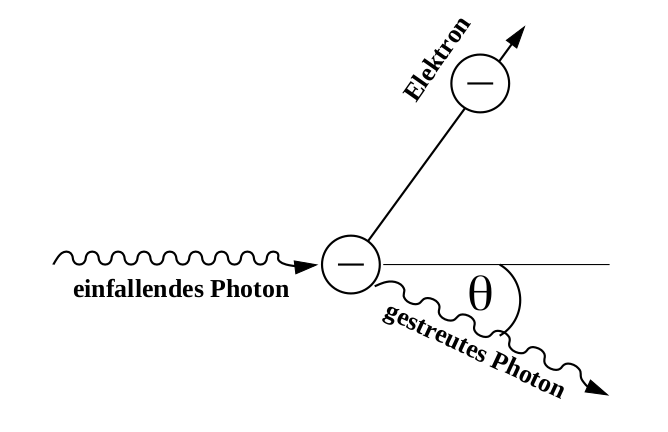
\includegraphics[width=0.4\textwidth]{images/bild_1.png}
    \caption{Schematische Darstellung des Compton Effekts.\cite{V603}}
    \label{fig:compton}
\end{figure}

Um den Effekt beobachten zu können wird hier Röntgenstrahlung an Plexiglas gestreut. 
Die ausfallende Strahlung wird über ein Geiger-Müller-Zählrohr und über die Transmission durch eine Aluminiumplatte mit der einfallenden Strahlung verglichen.
Diese Röntgenstrahlung wird in einer Röntgenröhre erzeugt, in der Elektronen von einer Glühkathode auf eine Anode beschleunigt werden. 
Der Zusammenstoß auf der Anode erzeugt $\gamma$-Strahlung.

Das Spektrum dieser Strahlung hängt vom Material der Anode ab.
Dieses ist zwar kontinuierlich, allerdings sind zwei Maxima in der Intensität deutlich zu erkennen, da diese Photonenenergien gerade der Energiedifferenz der Energieniveaus eines Anodenatoms entspricht.

Um die Wellenlänge $\lambda$ mit einer Photonenenergie in Verbindung zu bringen wird 
\begin{equation}
    E = \frac{h c}{\lambda}
    \label{eq:photonenenergie}
\end{equation} 
verwendet.

Um das charakteristische Spektrum der hier verwendeten Kupferanode zu bestimmen, wird die Röntgenstrahlung an einem LiF-Kristall gebeugt.
Hierbei entsteht beim Glanzwinkel $\alpha$ eine konstruktive Interferenz, welche von der Wellenlänge der Röntgenstrahlung abhängt. 
Die zugehörige Wellenlänge zum Winkel $\alpha$ kann über 
\begin{equation}
    \lambda = \frac{2d}{n}\sin\alpha
    \label{eq:glanzwinkel}
\end{equation}
bestimmt werden. 
Hier ist $d$ die Gitterkonstante des Kristalls und $n$ die Beugungsordnung.

Der Geiger-Müller-Zähler kann die Strahlung nicht kontinuierlich messen, sondern hat eine Totzeit $\tau$.
Daher muss dies über
\begin{equation}
    I = \frac{N}{1 - \tau N}
    \label{eq:totzeit}
\end{equation}
korrigiert werden. Hier ist $N$ die Anzahl der Anschläge des Geiger-Müller-Zählers und $I$ die Intensität der Strahlung.\cite{V603}
\section{Durchführung}
\label{sec:Durchführung}

% Was wurde gemessen bzw. welche Größen wurden variiert?

\subsection{Aufname der Geiger-Müller Charakterisik}
\label{ssec:d1}

Für die Messungen wird eine Schaltung wie in \autoref{fig:aufbau} aufgebaut.
Auf dem Zähldraht im Geiger-Müller-Zählrohr sammelt sich die Ladung $Q$, diese fließt dann über den Widerstand $R$ ab und erzeugt eine Spannung.
Diese Spannung wird vom Kondensator $C$ ausgekoppelt und daraufhin verstärkt, damit sie dann im Zähler gemessen werden kann.


\begin{figure}
    \centering
    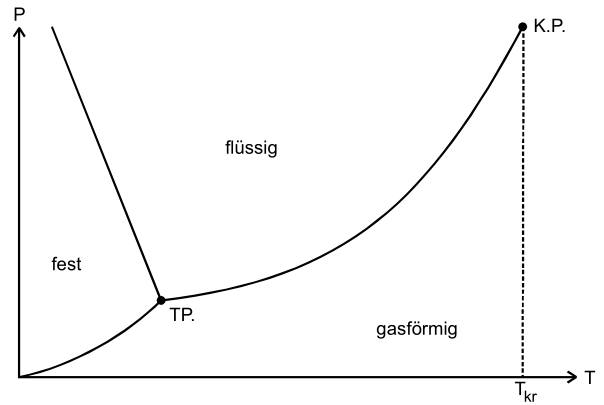
\includegraphics[width=\textwidth]{images/bild1.png}
    \caption{Aufbau der Messaperatur}
    \label{fig:aufbau}
\end{figure}

Nun wird eine Thallium-204-Quelle vor das Zählrohr gestellt, ein $\beta$ -Strahler.
Es ist wichtig zu beachten, dass alles so aufgebaut wird, dass die Zählrate nicht $\SI{100}{\text{Imps}\per\second}$ übersteigt.
Das wird getan, damit eine Totzeitkorrerkur nicht notwendig ist.
Die Zählrohrspannung $U$ wird auf $\SI{320}{\volt}$ gesetzt und es werden für je $\SI{60}{\second}$ die Impulse gemessen.
Dann wird die Spannung um $\SI{10}{\volt}$ vergrößert und erneut gemessen.
Dieser Vorgang wird bis einschließlich $\SI{700}{\volt}$ wiederholt.
Alle Daten werden notiert.

\subsection{Bestimmung der Totzeit}
\label{ssec:d2}

Um die gemessenen Impulse unter einer Totzeitkorrektur anspassen zu können, muss zunächst der Wert für die Totzeit berechnet werden.
Zunächst wird die Thallium-204-Quelle näher an das Zählrohr gerückt, da die Intensität hoch genug steigen muss, damit eine Korrektur nötig wird.
Dann werden mit einer Integrationszeit von $\SI{120}{\second}$ die Impulse gemessen.
Zusätzlich wird eine zweite Quelle verwendet.
Für diese wird die gleiche Messung durchgeführt, wie für die erste.
Abschließend wird noch eine Messung mit beiden Quellen durchgeführt.
Wichtig ist, dass die Abstände der Quellen zum Zählrohr jeweils gleich bleiben, da es sonst die Messung verfälscht.
Die drei Werte für die Intensitäten werden notiert.

\subsection{Bestimmung der freigesetzten Ladungen pro Teilchen}
\label{ssec:d3}

Die Messung für diesen Teil kann ebneso zusammen mit \autoref{ssec:d1} durchgeführt werden.
Es muss lediglich ab $\SI{350}{\volt}$ an, alle $\SI{50}{\volt}$ die Stromstärke $I$ abgelesen werden.
Dabei hat das Amperemeter eine Ablesegenauigkeit von $\SI{0.05}{\micro\ampere}$.
\newpage
\section{Auswertung}
\label{sec:Auswertung}

% Messwerte: Alle gemessenen physikalischen Größen sind übersichtlich darzustellen.

% Auswertung:
% Berechnung der geforderten Endergebnisse
% mit allen Zwischenrechnungen und Fehlerformeln, sodass die Rechnung nachvollziehbar ist.
% Eine kurze Erläuterung der Rechnungen (z.B. verwendete Programme)
% Graphische Darstellung der Ergebnisse

Auch die Auswertung ist, ähnlich wie die Durchführung, in 4 Teile aufgeteilt:
\begin{itemize}
    \item Überprüfung der Bragg Bedingung
    \item Untersuchung des Emissionsspektrums von Kuper
    \item Untersuchung der Absorptionsspektren verschiedener Materialien
    \item Bestimmung der Rydbergenergie
\end{itemize}



\subsection{Überprüfung der Bragg Bedingung}
\label{ssec:bragg_auswertung}

Die Messergebnisse aus Teil 1 der Durchführung sind in \autoref{tab:bragg} aufgelistet und in \autoref{fig:plot_bragg} dargestellt.
Die Maximale Intensität ergibt sich bei einem Winkel $\theta=\SI{28.2+-0.1}{\degree}$, wobei der Sollwinkel $\SI{28}{\degree}$ beträgt.

\begin{figure}
    \centering
    \includegraphics[width=\textwidth]{build/plot_bragg.pdf}
    \caption{Plot der Messergebnisse aus Abschnitt \ref{ssec:bragg}}
    \label{fig:plot_bragg}
\end{figure}



\subsection{Untersuchung des Emissionsspektrums von Kuper}
\label{ssec:emission_auswertung}

Die Messergebnisse aus Teil 2 der Durchführung sind in \autoref{tab:emission} aufgelistet und in \autoref{fig:plot_emission} dargestellt.
Hier lassen sich die $K$-Linien bei
\begin{align*}
    \theta(K_\alpha) &= \SI{22.5}{\degree} \\
    \theta(K_\beta) &= \SI{20.2}{\degree}
\end{align*}
ablesen und ergeben über \autoref{eq:bragg} und \ref{eq:energie} die Bindungsenergien
\begin{align*}
    E(K_\alpha) &= \SI{8044.2}{\electronvolt} \\
    E(K_\beta) &= \SI{8915.1}{\electronvolt} \,.
\end{align*}

\begin{figure}
    \centering
    \includegraphics[width=\textwidth]{build/plot_emission.pdf}
    \caption{Plot der Messergebnisse aus Abschnitt \ref{ssec:emission}}
    \label{fig:plot_emission}
\end{figure}

Nun soll das Auflösungsvermögen $A(K)=E(K)/H(K)$ der Röntgenstrahlung bestimmt werden, wobei $H(K)$ die Halbwärtsbreite der $K$-Linie ist.
Diese Halbwärtsbreite wird aufgrund der beschränkten Anzahl an Messpunkten um die $K$-Linien folgendermaßen bestimmt.
Zuerst werden die Messwerte gesucht, dessen Intensitätswerte am nächsten an $N(K)/2$ liegen.
Zwischen diesen Punkten wird jeweils eine Gerade gelegt.
Für diese Geraden wird der passende $\theta$ Wert für $N(K)/2$ bestimmt und wie zuvor über \autoref{eq:bragg} und \autoref{eq:energie} in eine Energie umgerechnet.
Die Differenzen dieser Energien ergeben somit die Halbwärtsbreiten
\begin{align*}
    H(K_\alpha) &= \SI{165.8}{\electronvolt} \\
    H(K_\beta) &= \SI{207.0}{\electronvolt}
\end{align*}
und die Auflösungsvermögen
\begin{align*}
    A(K_\alpha) &= \num{48.5} \\
    A(K_\beta) &= \num{43.1} \,.
\end{align*}

Außerdem werden aus den Energien $E(K)$ die Abschirmkonstanten $\sigma_1$ der Absorptionsenergie von Kupfer, $\sigma_2$ der $K_\alpha$-Linie und $\sigma_3$ der $K_\beta$-Linie bestimmt.
Da die Absorptionsenergie von Kuper hier nicht gemessen wurde, wird diese aus entsprechender Literatur zu $E_\text{abs}=\SI{8979}{\electronvolt}$ gewählt.\cite{absorption}
Abschätzungen der Abschirmkonstanten lassen sich über 
\begin{align}
    \sigma_1 &= Z - \sqrt{\frac{E_\text{abs}}{R_\infty}} \\
    \sigma_2 &= Z - \sqrt{4(Z-\sigma_1)^2-\frac{E(K_\alpha)}{R_\infty}} \\
    \sigma_3 &= Z - \sqrt{9(Z-\sigma_1)^2-\frac{E(K_\beta)}{R_\infty}}
\end{align}
ermitteln.\cite[Gleichungen (8),(9),(10)]{V602} 
Die Ordnungszahl von Kupfer ist $Z=29$.
Damit ergeben sich die Abschirmkonstanten zu
\begin{align*}
    \sigma_1 &= \num{3.3} \\
    \sigma_2 &= \num{12.4} \\
    \sigma_3 &= \num{22.5} \, .
\end{align*}



\subsection{Untersuchung der Absorptionsspektren verschiedener Materialien}
\label{ssec:absorption_auswertung}

Die Messergebnisse aus Teil 3 der Durchführung sind in den Tabellen \ref{tab:zink}-\ref{tab:zirconium} aufgelistet und in \autoref{fig:plot_absorption} dargestellt.

\begin{figure}
    \centering
    \includegraphics[width=\textwidth]{build/plot_absorption.pdf}
    \caption{Plot der Messergebnisse aus Abschnitt \ref{ssec:absorption}, mit Markierungen der bestimmten $K$-Kanten}
    \label{fig:plot_absorption}
\end{figure}

Aus den Messdaten kann nun jeweils die Absorptionsenergie bestimmt werden.
Dazu wird die $K$-Kante näherungsweise auf die Mitte der Kante festgelegt.
Also wird der nächstbeste $\theta$ Wert zu $N=N_\text{min} + \frac{1}{2}(N_\text{max}-N_\text{min})$ bestimmt bzw. die Mitte zweier Messwerte falls die Gesuchte Intensität ungefähr in der Mitte dieser Messpunkte liegt.
Die so gefundenen $K$-Kanten sowie deren Energieäquivalent aus \autoref{eq:bragg} und \ref{eq:energie} sind in \autoref{tab:absorption} aufgelistet.

Nun kann aus den Absorptionsenergien über \autoref{eq:abschirm} die Abschirmkonstanten der Absorbermaterialien bestimmt werden.

Um die bestimmten Werte vergleichen zu können, werden über Absorptionsenergien aus externer Literatur und die gleichen drei Gleichungen wie zuvor Abschirmkonstanten und die Bragg-Winkel berechnet.
Auch diese Werte sind in \autoref{tab:absorption} aufgelistet.

\begin{table}
    \centering
    \caption{Ergebnisse und Literaturwerte der Absorptionsenergie, des Bragg-Winkels und der Abschirmkonstante.\cite{absorption}}
    \sisetup{
        table-format=2.2
    }
    \begin{tabular}{c S[table-format=1.0] S S S S S S}
        \toprule
        Element & $Z$ & \tableSI{E}{\kilo\electronvolt} & \tableSI{E_\text{Lit}}{\kilo\electronvolt} & \tableSI{\theta}{\degree} & \tableSI{\theta_\text{Lit}}{\degree} & $\sigma$ & $\sigma_\text{Lit}$ \\
        \midrule
        Zn & 30 & 9.60 & 9.65 & 18.70 & 18.60 & 3.63 & 3.57 \\
        Ga & 31 & 10.32 & 10.37 & 17.35 & 17.30 & 3.67 & 3.61 \\
        Br & 35 & 13.43 & 13.47 & 13.25 & 13.20 & 3.89 & 3.85 \\
        Rb & 37 & 15.05 & 15.20 & 11.80 & 11.70 & 4.11 & 3.94 \\
        Sr & 38 & 15.99 & 16.10 & 11.10 & 11.00 & 4.12 & 4.00 \\
        Zr & 40 & 17.73 & 18.00 & 10.00 & 9.80 & 4.37 & 4.09 \\
        \bottomrule
    \end{tabular}
    \label{tab:absorption}
\end{table}



\subsection{Bestimmung der Rydbergenergie}
\label{ssec:rydberg}

Nun lässt sich aus den im vorherigen Abschnitt berechneten Absorptionsenergien sowie Abschirmkonstanten die Rydbergenergie über \autoref{eq:moseley} ermitteln.
Dazu wird ein Plot aus den Werten aus \autoref{tab:absorption} angefertigt und eine passende Ausgleichsgerade mit
\begin{equation*}
    \sqrt{E} = aZ+b
\end{equation*}
über die Python Funktion curve\_fit aus der Bibliothek Scipy bestimmt.
Somit ergeben sich die Parameter
\begin{align*}
    a &= \SI{3.52+-0.02}{\sqrt{\electronvolt}} \\
    b &= \SI{-7.6+-0.7}{\sqrt{\electronvolt}} \,.
\end{align*}

\begin{figure}
    \centering
    \includegraphics[width=\textwidth]{build/plot_rydberg.pdf}
    \caption{Plot der Ergebnisse aus \autoref{tab:absorption} mit passender Ausgleichsgerade.}
    \label{fig:plot_rydberg}
\end{figure}

Die Rydbergenergie wird über $R_\infty=a^2$ zu 
\begin{equation*}
    R_\infty = \SI{12.4+-0.1}{\electronvolt}
\end{equation*}
bestimmt.

Ein Literaturwert der Rydbergenergie lautet $R_\infty=\SI{13.6}{\electronvolt}$.\cite{V602}
\section{Diskussion}
\label{sec:Diskussion}

% Kurze Zusammenfassung der Ergebnisse
% -Vergleich mit Literaturwerten
% -Vergleich mit verschiedenen Messverfahren
% -bei Abweichungen mögliche Ursachen finden

Es ergeben sich also insgesamt vier verschiedene Elastizitätsmodule $E$ für 2 verschiedene Metalle. 

\printbibliography{}

\begin{figure}
    \centering
    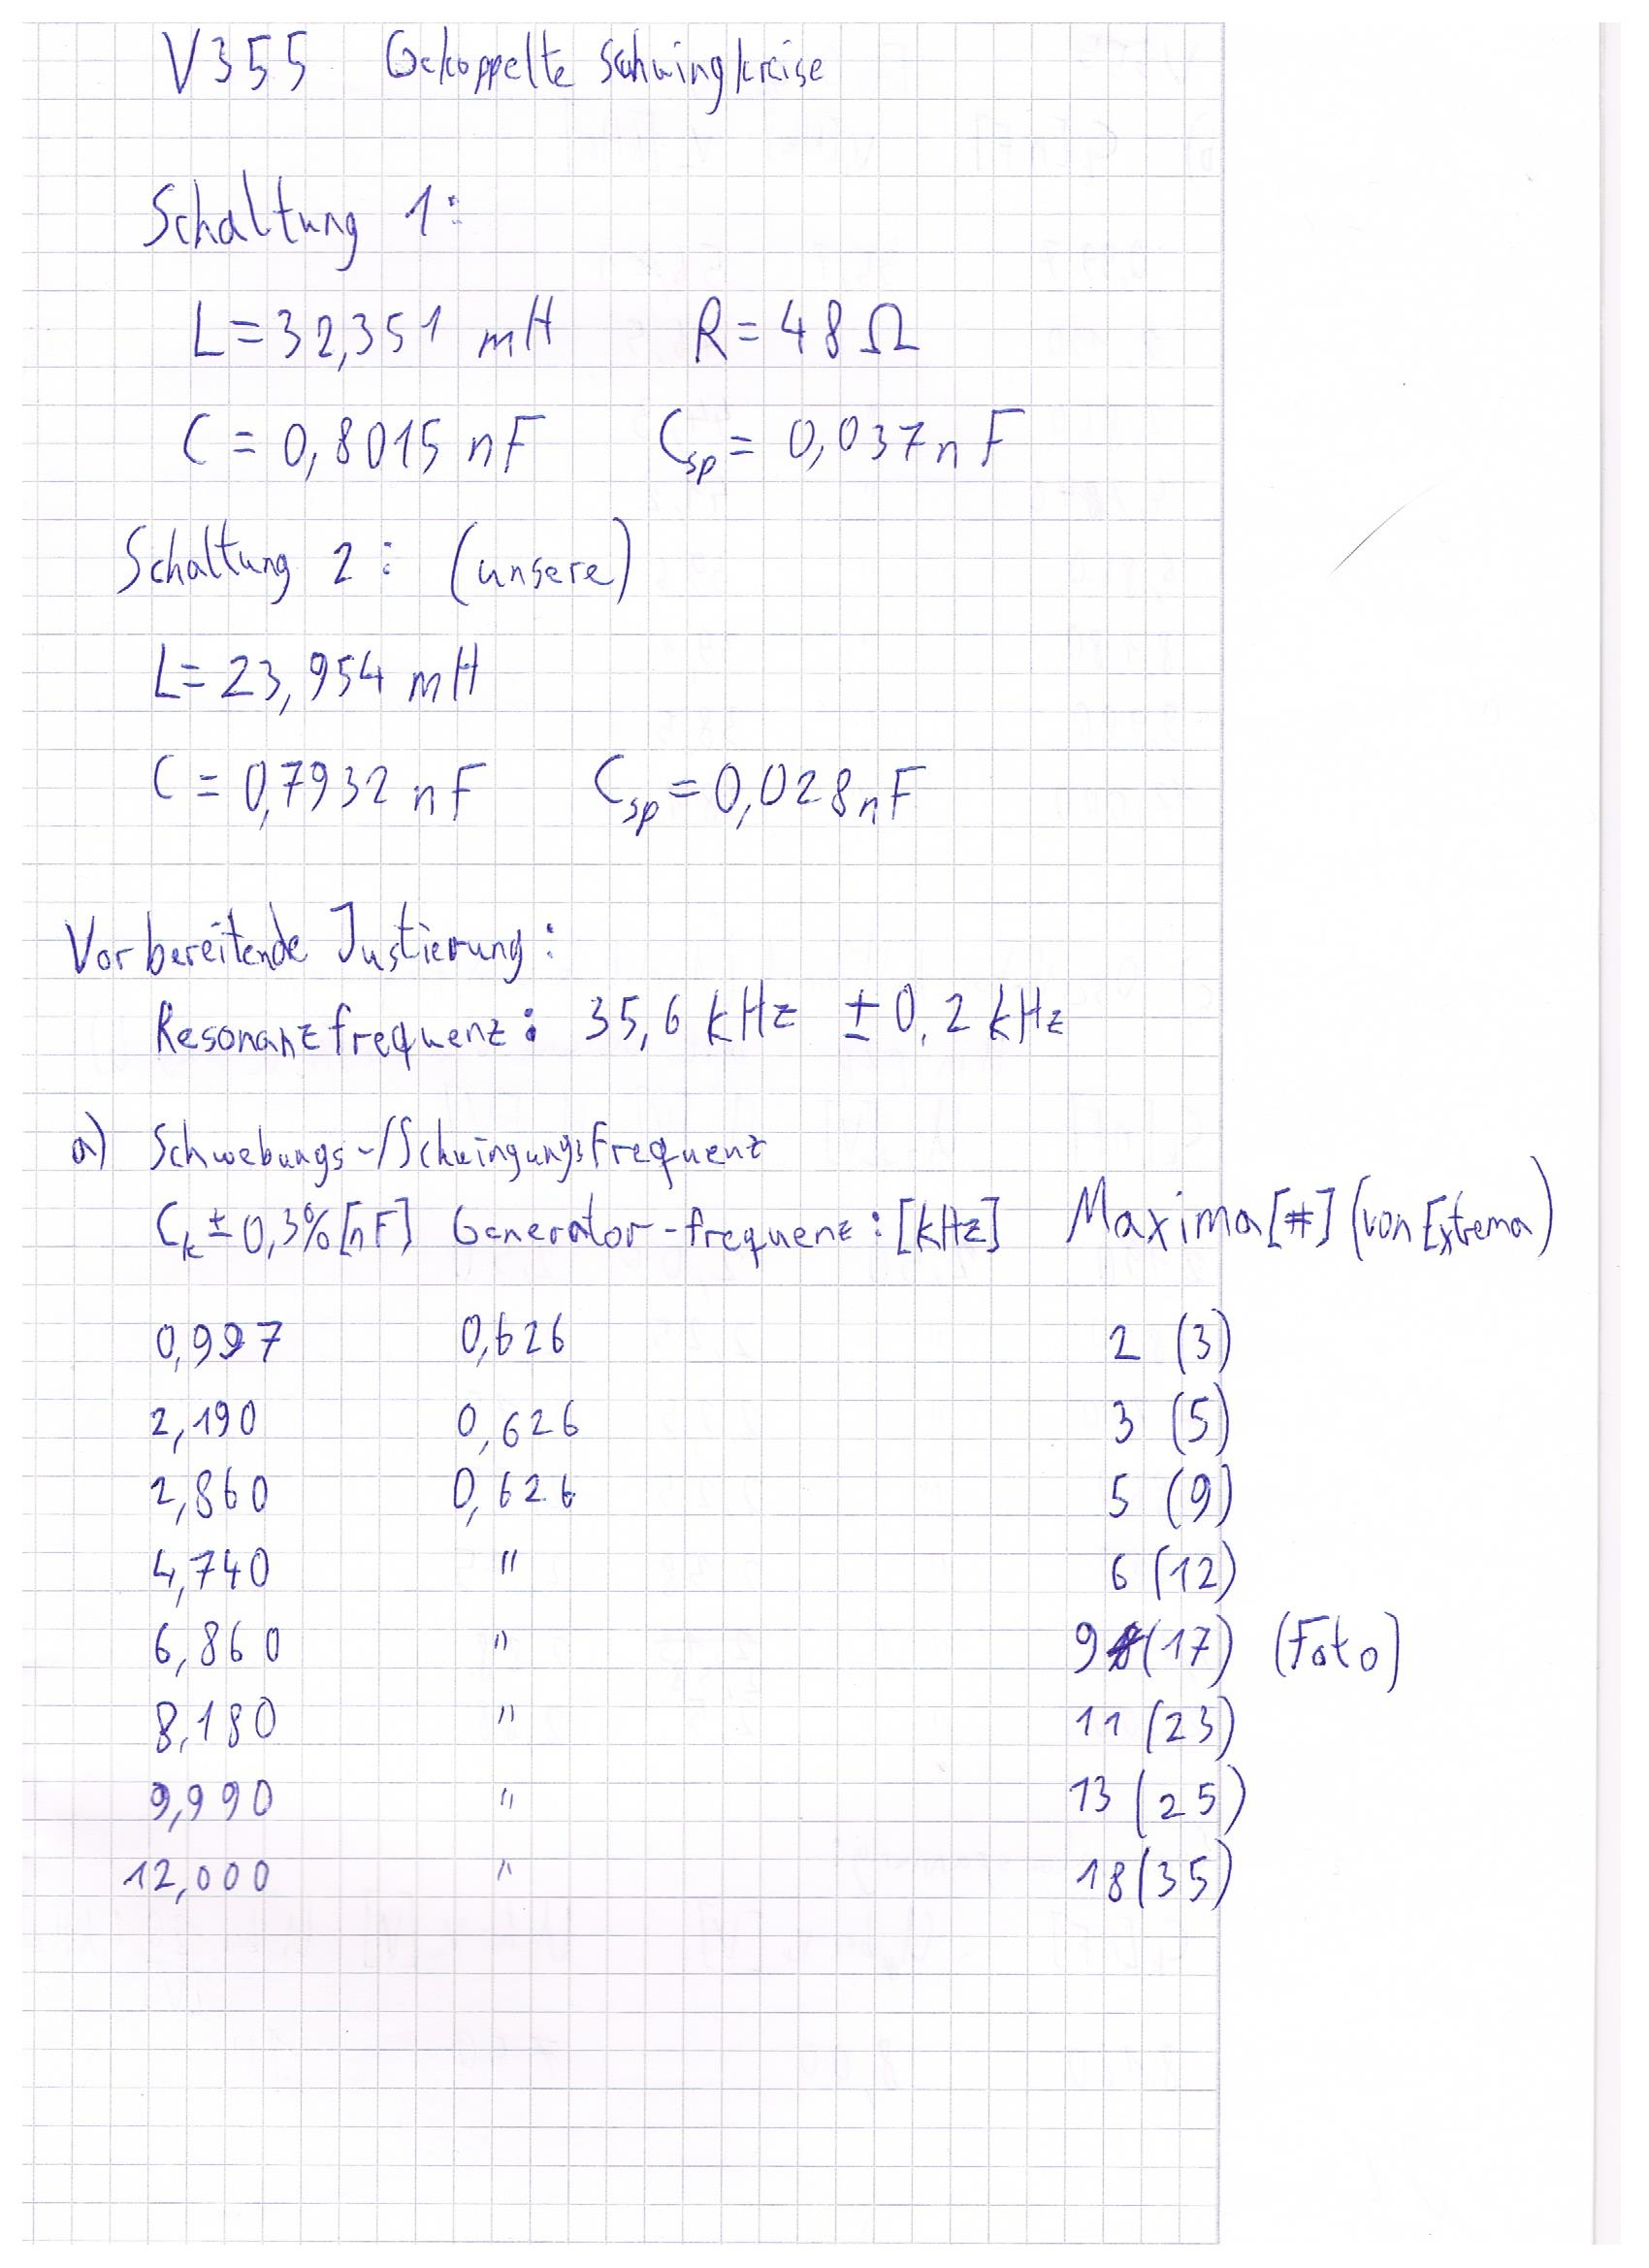
\includegraphics[width=\textwidth]{images/originaldaten_1.png}
    \caption{Seite 1 der Originalmessdaten}
    \label{fig:originaldaten_1}
\end{figure}
\begin{figure}
    \centering
    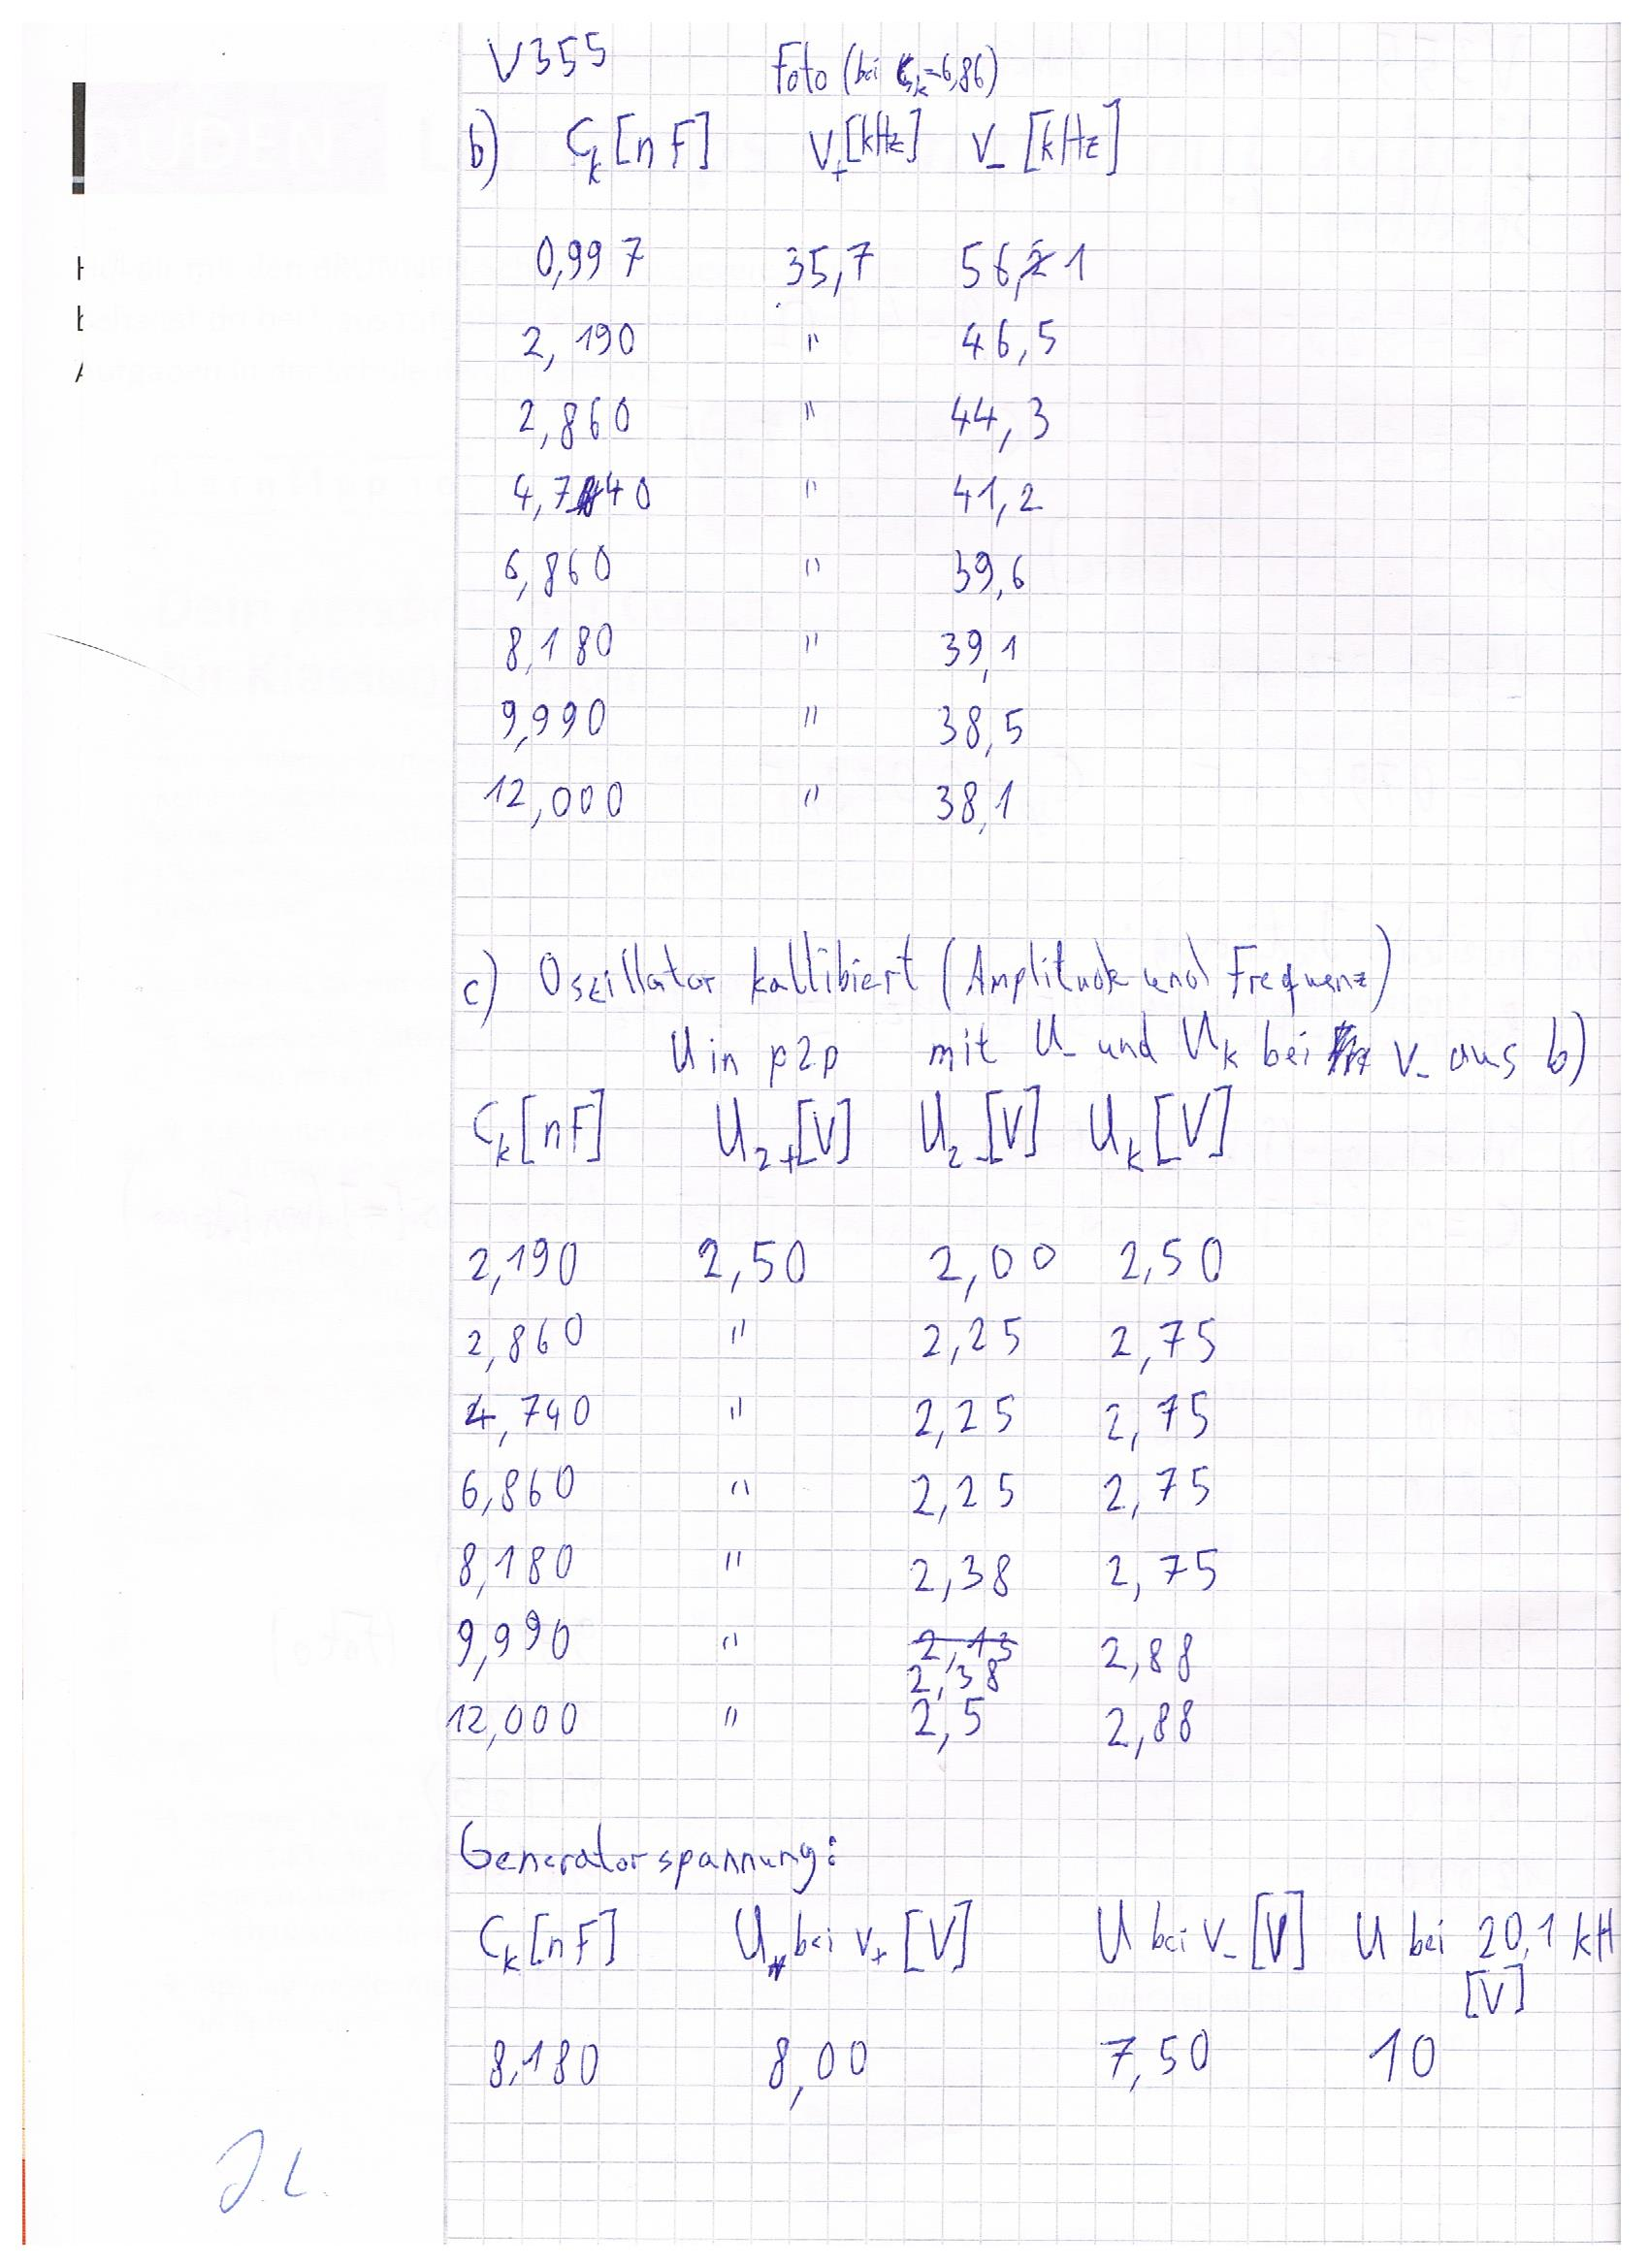
\includegraphics[width=\textwidth]{images/originaldaten_2.png}
    \caption{Seite 2 der Originalmessdaten}
    \label{fig:originaldaten_2}
\end{figure}

\end{document}
